%  ALWAYS USE THE referee OPTION WITH PAPERS SUBMITTED TO BIOMETRICS!!!
%  You can see what your paper would look like typeset by removing
%  the referee option.  Because the typeset version will be in two
%  columns, however, some of your equations may be too long. DO NOT
%  use the \longequation option discussed in the user guide!!!  This option
%  is reserved ONLY for equations that are impossible to split across 
%  multiple lines; e.g., a very wide matrix.  Instead, type your equations 
%  so that they stay in one column and are split across several lines, 
%  as are almost all equations in the journal.  Use a recent version of the
%  journal as a guide. 
%  
\documentclass[useAMS,referee]{biom}
\usepackage{amsmath}
\usepackage{bbm}
\usepackage{dsfont}
\usepackage{graphicx}
\usepackage{blindtext}
\usepackage{booktabs}
\usepackage{breqn}
\usepackage{algorithm}
\usepackage{algcompatible}
\usepackage{algpseudocode}
\usepackage{float}
\usepackage{dutchcal}
\usepackage{amsfonts}




\let\origfigure\figure
\let\endorigfigure\endfigure
\renewenvironment{figure}[1][2] {
    \expandafter\origfigure\expandafter[H]
} {
    \endorigfigure
}


\def\bSig\mathbf{\Sigma}
\newcommand{\VS}{V\&S}
\newcommand{\tr}{\mbox{tr}}

%  Here, place your title and author information.  Note that in 
%  use of the \author command, you create your own footnotes.  Follow
%  the examples below in creating your author and affiliation information.
%  Also consult a recent issue of the journal for examples of formatting.

\title[]{Bayesian multivariate skew-normal finite mixture model for analysis of infant development trajectories}

%  Here are examples of different configurations of author/affiliation
%  displays.  According to the Biometrics style, in some instances,
%  the convention is to have superscript *, **, etc footnotes to indicate 
%  which of multiple email addresses belong to which author.  In this case,
%  use the \email{ } command to produce the emails in the display.

%  In other cases, such as a single author or two authors from 
%  different institutions, there should be no footnoting.  Here, use
%  the \emailx{ } command instead. 

%  The examples below corrspond to almost every possible configuration
%  of authors and may be used as a guide.  For other configurations, consult
%  a recent issue of the the journal.

%  Single author -- USE \emailx{ } here so that no asterisk footnoting
%  for the email address will be produced.

%\author{John Author\emailx{email@address.edu} \\
%Department of Statistics, University of Warwick, Coventry CV4 7AL, U.K.}

%  Two authors from the same institution, with both emails -- use
%  \email{ } here to produce the asterisk footnoting for each email address

%\author{John Author$^{*}$\email{author@address.edu} and
%Kathy Authoress$^{**}$\email{email2@address.edu} \\
%Department of Statistics, University of Warwick, Coventry CV4 7AL, U.K.}

%  Exactly two authors from different institutions, with both emails  
%  USE \emailx{ } here so that no asterisk footnoting for the email address
%  is produced.

\author
{Carter Allen\emailx{allecart@musc.edu} \\
Department of Public Health Sciences, Medical University of South Carolina, Charleston, SC, U.S.A
\and
Brian Neelon, PhD \\
Department of Public Health Sciences, Medical University of South Carolina, Charleston, SC, U.S.A
\and
Sara Benjamin-Neelon, PhD, MPH, RD \\
Department of Health, Behavior and Society, Johns Hopkins University, Baltimore, MD, U.S.A}

%  Three or more authors from same institution with all emails displayed
%  and footnoted using asterisks -- use \email{ } 

%\author{John Author$^*$\email{author@address.edu}, 
%Jane Author$^{**}$\email{jane@address.edu}, and 
%Dick Author$^{***}$\email{dick@address.edu} \\
%Department of Statistics, University of Warwick, Coventry CV4 7AL, U.K}

%  Three or more authors from same institution with one corresponding email
%  displayed

%\author{John Author$^*$\email{author@address.edu}, 
%Jane Author, and Dick Author \\
%Department of Statistics, University of Warwick, Coventry CV4 7AL, U.K}

%  Three or more authors, with at least two different institutions,
%  more than one email displayed 

%\author{John Author$^{1,*}$\email{author@address.edu}, 
%Kathy Author$^{2,**}$\email{anotherauthor@address.edu}, and 
%Wilma Flinstone$^{3,***}$\email{wilma@bedrock.edu} \\
%$^{1}$Department of Statistics, University of Warwick, Coventry CV4 7AL, U.K \\
%$^{2}$Department of Biostatistics, University of North Carolina at 
%Chapel Hill, Chapel Hill, North Carolina, U.S.A. \\
%$^{3}$Department of Geology, University of Bedrock, Bedrock, Kansas, U.S.A.}

%  Three or more authors with at least two different institutions and only
%  one email displayed

%\author{John Author$^{1,*}$\email{author@address.edu}, 
%Wilma Flinstone$^{2}$, and Barney Rubble$^{2}$ \\
%$^{1}$Department of Statistics, University of Warwick, Coventry CV4 7AL, U.K \\
%$^{2}$Department of Geology, University of Bedrock, Bedrock, Kansas, U.S.A.}


\begin{document}

%  This will produce the submission and review information that appears
%  right after the reference section.  Of course, it will be unknown when
%  you submit your paper, so you can either leave this out or put in 
%  sample dates (these will have no effect on the fate of your paper in the
%  review process!)

\date{{\it Received October} 2007. {\it Revised February} 2008.  {\it
Accepted March} 2008.}

%  These options will count the number of pages and provide volume
%  and date information in the upper left hand corner of the top of the 
%  first page as in published papers.  The \pagerange command will only
%  work if you place the command \label{firstpage} near the beginning
%  of the document and \label{lastpage} at the end of the document, as we
%  have done in this template.

%  Again, putting a volume number and date is for your own amusement and
%  has no bearing on what actually happens to your paper!  

\pagerange{\pageref{firstpage}--\pageref{lastpage}} 
\volume{64}
\pubyear{2008}
\artmonth{December}

%  The \doi command is where the DOI for your paper would be placed should it
%  be published.  Again, if you make one up and stick it here, it means 
%  nothing!

\doi{10.1111/j.1541-0420.2005.00454.x}

%  This label and the label ``lastpage'' are used by the \pagerange
%  command above to give the page range for the article.  You may have 
%  to process the document twice to get this to match up with what you 
%  expect.  When using the referee option, this will not count the pages
%  with tables and figures.  

\label{firstpage}

%  put the summary for your paper here

\begin{abstract}
In studies of infant motor development, a crucial research goal is the identification of latent clusters of infants who experience delayed motor development, as this is a known risk factor for adverse outcomes later in life. However, there are a number of statistical challenges in modeling infant motor development: the data are typically skewed, exhibit intermittent missingness, and are highly correlated across the repeated measurements collected during infancy. Using data from the Nurture study, a cohort of over 600 mother-infant pairs followed from pregnancy to 12 months postpartum, we develop a flexible Bayesian finite mixture model for the analysis infant motor development. Our model has a number of attractive features. First, we adopt the multivariate skew normal distribution with cluster-specific parameters that accommodate the inherent correlation and skewness in the data. Second, we model the cluster membership probabilities using a novel application of the P\'olya-Gamma data-augmentation scheme, thereby improving predictions of the cluster membership allocations. Lastly, we impute missing responses under the missing at random assumption by drawing from appropriate conditional multivariate skew  normal distributions. Bayesian inference is achieved through straightforward Gibbs sampling, and can be implemented in available software such as \texttt{R}.  Through simulation studies, we show that the proposed model yields improved inferences over models that ignore skewness. In addition, our imputation method yields improvements compared to conventional missing data methods, including multiple imputation and complete or available case analysis. When applied to Nurture data, we identified two distinct development clusters: one characterized by delayed “U-shaped” motor development and a higher percentage of male infants and another characterized by more steady motor development and a lower percentage of males. The clusters also differed in terms of key demographic variables, such as infant race and maternal pre-pregnancy body mass index. These findings can aid investigators in targeting interventions during this critical early-life developmental window.
\end{abstract}

%  Please place your key words in alphabetical order, separated
%  by semicolons, with the first letter of the first word capitalized,
%  and a period at the end of the list.
%

\begin{keywords}
Mixture of Experts, P\'olya-Gamma, Skew-Normal, Imputation, Latent Growth, Infant Development.
\end{keywords}

%  As usual, the \maketitle command creates the title and author/affiliations
%  display

\maketitle

\setcounter{tocdepth}{3}
\tableofcontents

\newpage

%  If you are using the referee option, a new page, numbered page 1, will
%  start after the summary and keywords.  The page numbers thus count the
%  number of pages of your manuscript in the preferred submission style.
%  Remember, ``Normally, regular papers exceeding 25 pages and Reader Reaction 
%  papers exceeding 12 pages in (the preferred style) will be returned to 
%  the authors without review. The page limit includes acknowledgements, 
%  references, and appendices, but not tables and figures. The page count does 
%  not include the title page and abstract. A maximum of six (6) tables or 
%  figures combined is often required.''

%  You may now place the substance of your manuscript here.  Please use
%  the \section, \subsection, etc commands as described in the user guide.
%  Please use \label and \ref commands to cross-reference sections, equations,
%  tables, figures, etc.
%
%  Please DO NOT attempt to reformat the style of equation numbering!
%  For that matter, please do not attempt to redefine anything!

\section{Introduction}
\label{s:intro}

\subsection{Infant Development Clustering}

Heterogeneity of treatment effects (HTE) (Lanza and Rhoades, 2013). 

\subsection{Existing Approaches}

Mixtures of multivariate non-symmetric distributions such as the multivariate skew-normal (MSN) distribution allow for the nuances of the marginal density to be captured with a more parsimonious set of mixture components. Mixtures of MSN distributions have been dealt with previously in a Bayesian context (Fr\"{u}hwirth-Schnatter \& Pyne, 2010 and others), however in these models, focus lies primary on marginal density estimation, and inference on the mixture components (i.e. clusters) is often not discussed. More recently, the mixtures of skew-$t$ factor analysis (MSTFA) model has been proposed for settings in which cluster-specific inference is of primary interest (Lin \textit{et al.} 2018). However, an important feature not included in the MSTFA is the ability to explain individual-level cluster membership as a function of covariates of interest. Additionally, the parameter estimation procedure proposed by Lin et al. for the MSTFA relies on a prohibitively complex EM algorithm and does not enjoy the inferential benefits of a Bayesian approach, including the ability to incorporate prior information into a model and make posterior probability statements. Our proposed model improves on these previous works by estimating parameters in a Bayesian framework as well as including the ability to fit a multinomial logit regression to cluster membership probabilities using a novel application of data augmentation with the P\'olya-Gamma distribution.

Polson et al. (2013) introduce a data augmentation scheme using the P\'olya-Gamma distribution which allows for sampling of multinomial regression parameters using straightforward Gibb's updates from Gaussian full conditional distributions. In addition to more convenient parameter estimation, the P\'olya-Gamma data augmentation method for logistic regression has the advantage of direct sampling from the posterior distributions of multinomial parameters. This approach avoids the need for approximations of the posterior distribution, thus yielding more stable sampling, especially when the number of parameters approaches the number of observations (Polson et al., 2013). P\'olya-Gamma data augmentation for multinomial regression has not yet been applied to the analysis of longitudinally clustered data. 

A ubiquitous feature of repeated measures studies is loss of data due to intermittent missingness and attrition. In the Bayesian setting, the standard approach to dealing with missing data is to perform multiple imputation, whereby $M$ imputed data sets are generated from a specified imputation model. After $M$ complete data sets are obtained, parameter estimates are combined across each data set to produce a final set of parameter estimates (Gelman \textit{et al.} 2013). This approach is not only computationally burdensome, requiring storage and analysis of an $M \times n_{rows} \times n_{cols}$ data array in addition to multiplication of total model run time by a factor of $M$, but it has been shown to produce unreliable inferences (Zhou and Reiter, 2010). We instead include an ``online" imputation imputation step in our Gibbs sampling procedure, whereby missing outcomes are updated at each iteration. This approach greatly increases the number of opportunities for exploration of the missing data parameter space and avoids the multiplication of total run time and number of parameters.

\newpage

\section{Nurture Study}
\label{s:nurt}
\subsection{Baseline Demographics and Description of Variables}

\subsection{Statistical Challenges}

The analysis of infant motor development trends in the Nurture data presents a number of statistical challenges that motivate our proposed model. First, as depicted in Figure 1, the residuals from repeated measures models of Bayley composite scores exhibit skewness even after adjusting for covariates such as race, sex, and birthweight. This suggests that the assumption of conditional normality made by standard repeated measures models is violated, and a distinguishing feature of the data, skewness, is not being accounted for. 

\begin{figure}[h]
	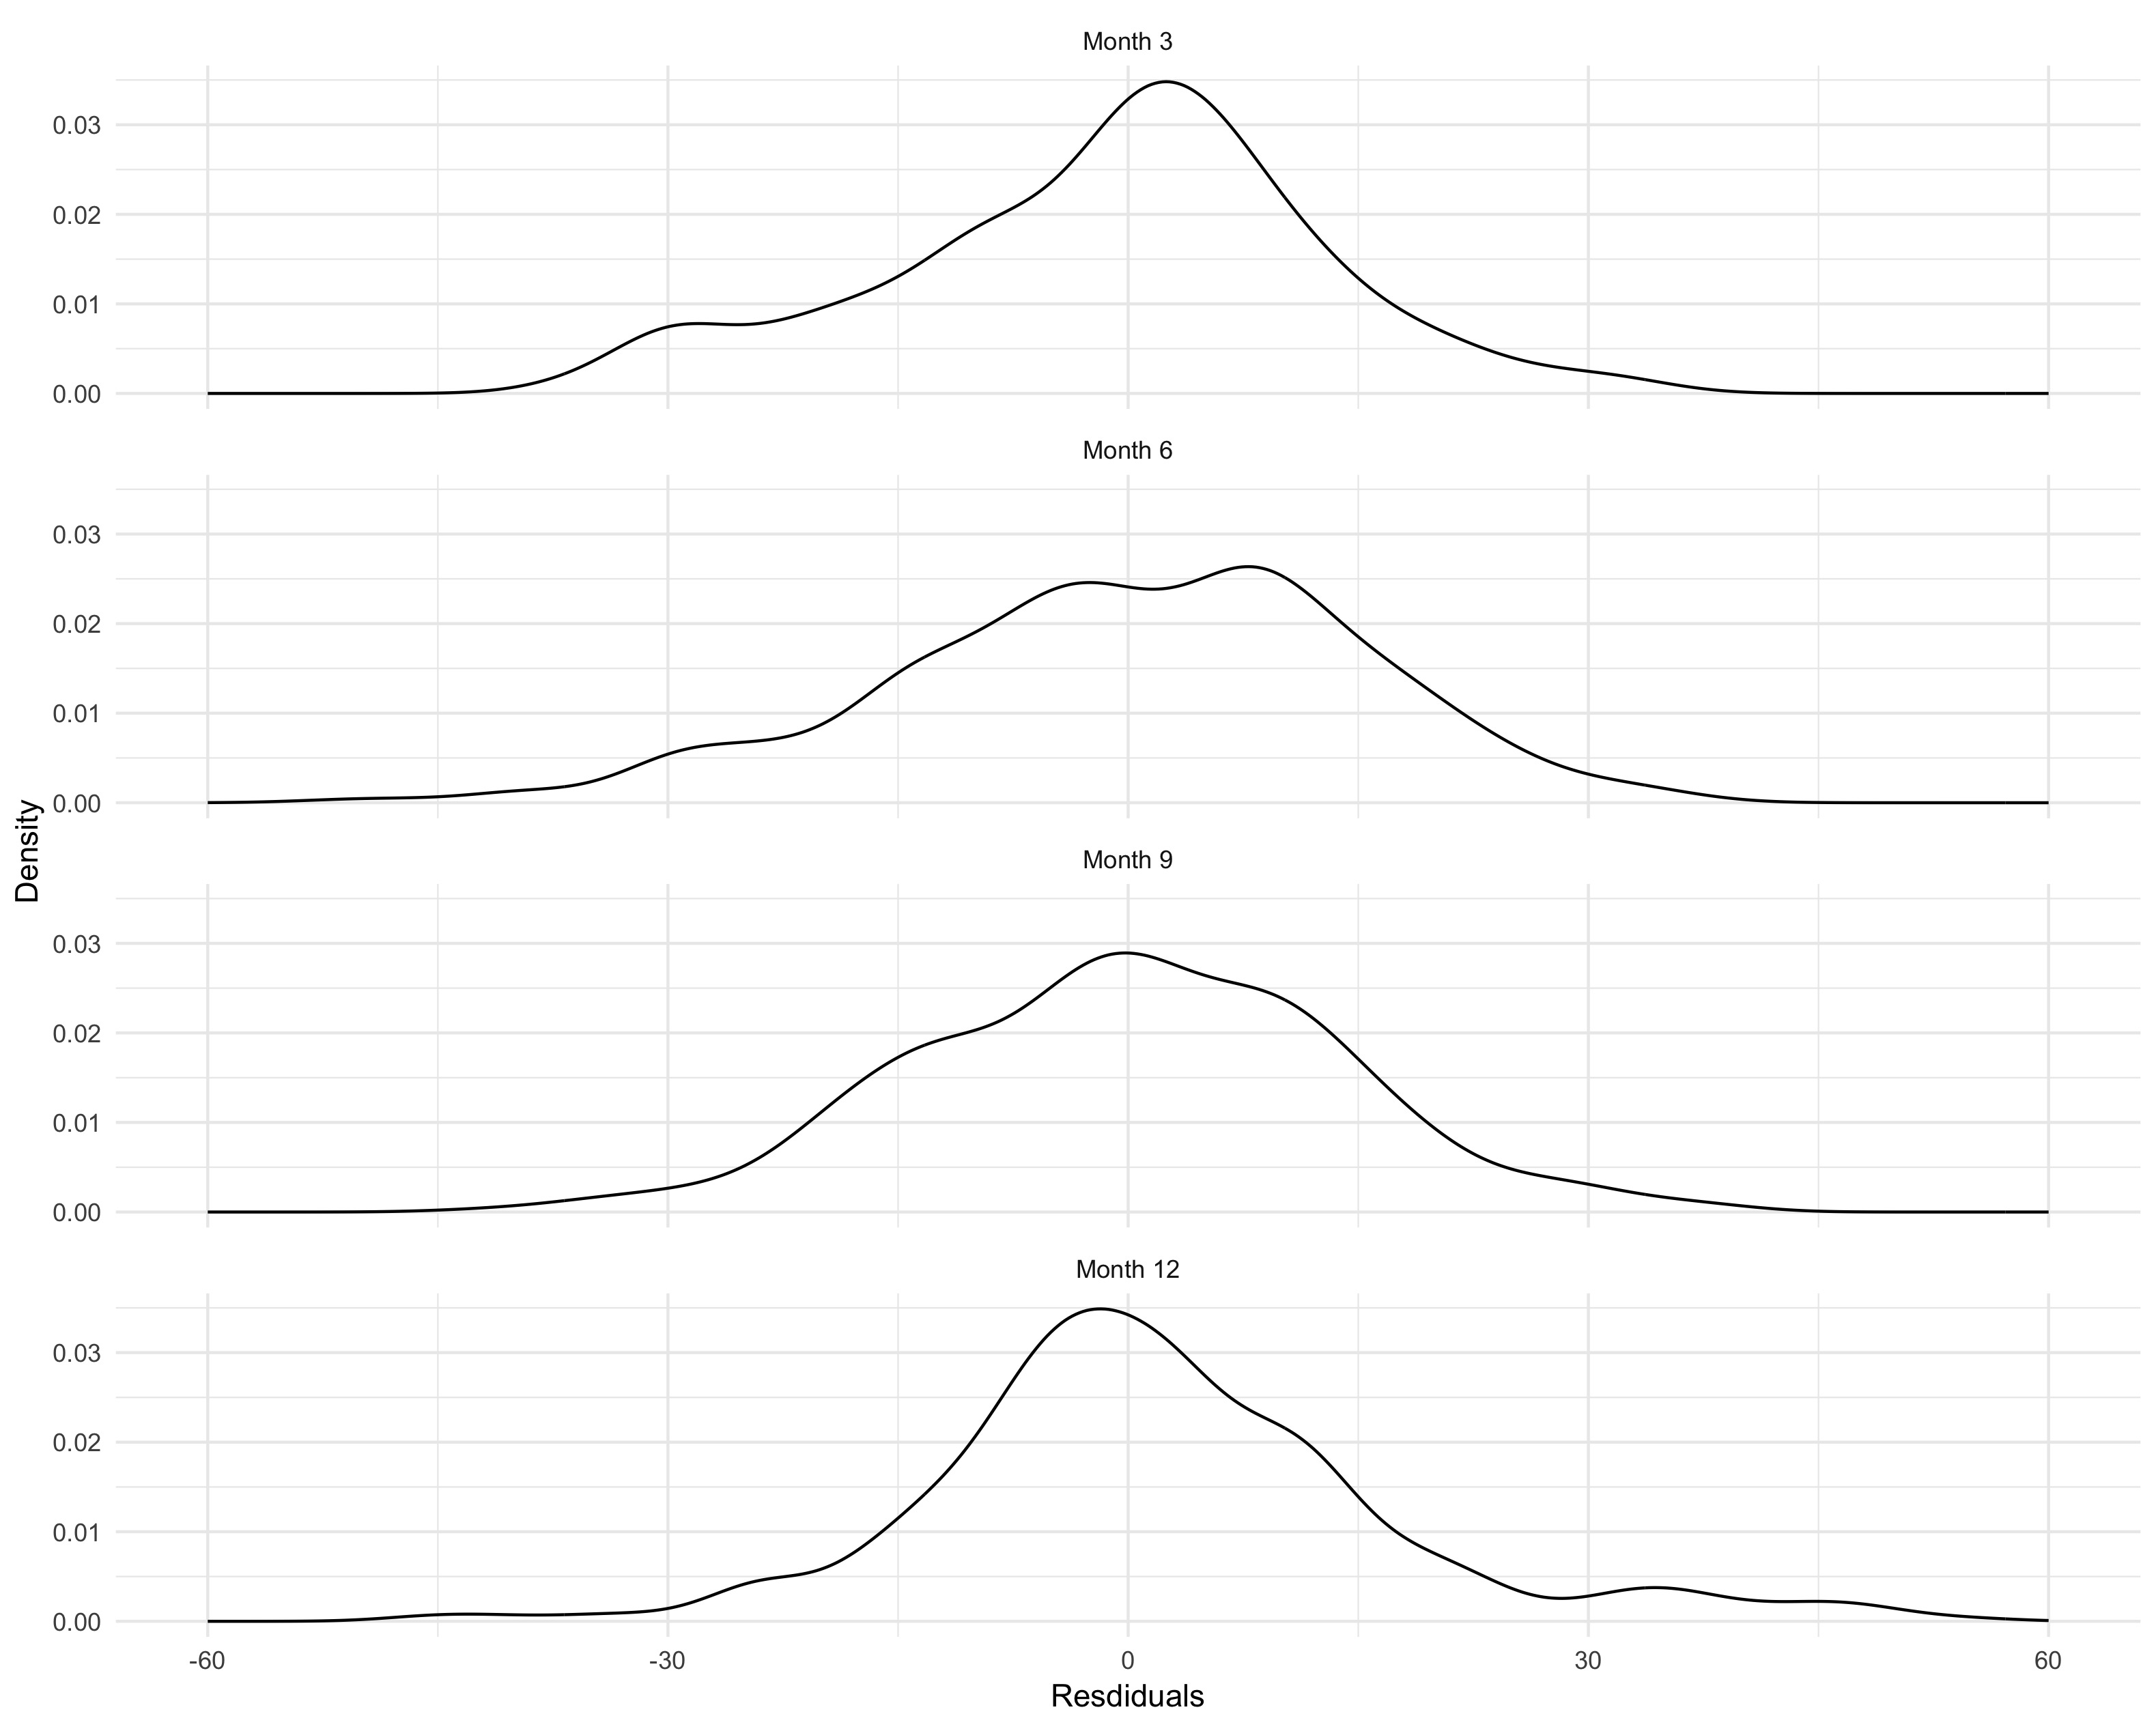
\includegraphics[width = 1\textwidth]{bayley_resids_plot_bytime.jpg}
\end{figure}

The Nurture data also feature intermittent missingness in Bayley composite scores throughout the study period. Of the total cohort (N = 666), 429 (64.4 \%) observations were available at three months, 435 (65.3 \%) observations were available at six months, 418 (62.8 \%) observations were available at nine months, and 437 (65.6 \%) observations were available at twelve months. As such, we require a modeling framework capable of dealing with missing data. 


\section{Model}
\label{s:model}

\subsection{Multivariate Skew Normal Mixture Model}

A primary goal of the Nurture study is to identify clusters of infants characterized by distinct motor development trajectories throughout the first year of life. To address this aim, we propose a flexible finite mixture model that accommodates relevant features of the data, such as skewness, missing values, and dependence among the responses. For $i = 1,...,n$, let $\mathbf{y}_{i}=(y_{i1},\ldots,y_{iJ})^T$ be a $J \times 1$ vector of responses (i.e., Bayley composite scores) for subject $i$ across the $J$ measurement occasions. For analysis of the Nurture data, we propose a finite mixture model of the form
\begin{equation}
	\label{eq:mixture}
f(\mathbf{y}_i) = \sum_{k = 1}^{K} \pi_{ki} f(\mathbf{y}_i|\boldsymbol\theta_k),
\end{equation}
where $\boldsymbol\theta_k$ is the set of parameters specific to cluster $k$ ($k = 1,...,K$) and $\pi_{ki}$ is a subject-specific mixing weight representing the probability that subject $i$ belongs to cluster $k$. For now we assume that $K$ is fixed; in Section \ref{s:mcmcmisc}, we discuss model selection strategies for choosing the optimal value of $K$. 

To facilitate posterior inference, we introduce a latent cluster indicator variable $z_i$ taking the value $k \in \{1,...,K\}$ with probability $\pi_{ki}$. Conditional on $z_i = k$, we assume $\mathbf{y}_{i}$ is distributed as
\begin{equation}
\mathbf{y}_{i}|(z_i=k) \sim \text{MSN}_J(\boldsymbol\zeta_{ki},\boldsymbol\alpha_k,\boldsymbol\Omega_k), \label{eq:msndens}
\end{equation}
where $\text{MSN}_J(\cdot)$ denotes the $J$-dimensional multivariate skew normal density, $\boldsymbol\zeta_{ki}$ is a $J \times 1$ vector of subject- and cluster-specific location parameters, $\boldsymbol\alpha_k$ is a $J \times 1$ vector of cluster-specific skewness parameters, and $\boldsymbol\Omega_k$ is a $J \times J$ cluster-specific scale matrix that captures dependence among the $J$ responses for subject $i$. The vector $\boldsymbol\alpha_k$ has components $\alpha_{kj}$, $j = 1,...,J$, that control the skewness of outcome $j$ in cluster $k$. When $\boldsymbol\alpha_k = \mathbf{0}$, the MSN distribution reduces to the multivariate normal distribution $\text{N}_J(\boldsymbol\zeta_{ki},\boldsymbol\Omega_k)$, where $\boldsymbol\zeta_{ki}$ is a $J \times 1$ mean vector and $\boldsymbol\Omega_k$ is a $J \times J$ covariance matrix.

We can extend model (\ref{eq:msndens}) to the regression setting by modeling $\boldsymbol\zeta_{ki}$ as a function of covariates. Here we adopt a convenient stochastic representation of the MSN density (Azzalini and Dalla Valle, 1996):
\begin{equation}
\mathbf{y}_{i}|(z_i=k,t_i) = \mathbf{X}_i \boldsymbol\beta_k + t_i \boldsymbol\psi_k + \boldsymbol\epsilon_{ki}, \label{eq:msnreg}
\end{equation}
where 
$\mathbf{X}_i$ is a $J \times Jp$ design matrix that includes potential time-varying covariates (e.g., indicators denoting quarterly visits); $\boldsymbol{\beta}_k=(\beta_{k11},\ldots,\beta_{k1p},\ldots,\beta_{kJ1},\ldots,\beta_{kJp})^T$ is a $Jp\times 1$ vector of cluster- and outcome-specific regression coefficients; $t_i\sim \text{N}_{[0,\infty)}(0,1)$ is a subject-specific standard normal random variable truncated below by zero; $\boldsymbol\psi_k=(\psi_{k1},\ldots,\psi_{kJ})^T$ is a $J \times 1$ vector of cluster-specific skewness parameters; and $\boldsymbol{\epsilon}_{ki} \sim \text{N}_J(\boldsymbol0,\boldsymbol\Sigma_k)$ is a $J\times 1$ vector of correlated error terms. Thus, conditional on $t_i$ and $z_i=k$, $\boldsymbol{y}_i$ is distributed as $\text{N}_J(\mathbf{X}_i \boldsymbol\beta_k + t_i \boldsymbol\psi_k, \boldsymbol{\Sigma}_k)$. Marginally (after integrating over $t_i$), $\mathbf{y}_i|(z_i = k)$ is distributed $\text{MSN}_J(\boldsymbol\zeta_{ki}, \boldsymbol\alpha_k, \boldsymbol\Omega_k)$, where through back-transformation 
\begin{eqnarray}
\boldsymbol\zeta_{ki} &=& \mathbf{X}_i\boldsymbol\beta_k, \nonumber \\
\boldsymbol\alpha_k &=& \frac{1}{\sqrt{1 - \boldsymbol\psi_k^T 
\boldsymbol\Omega^{-1}_k\boldsymbol\psi_k}} \boldsymbol\omega_k \boldsymbol\Omega^{-1}_k\boldsymbol\psi_k,~~\text{and} \label{eq:back_transform}\\
\boldsymbol\Omega_k &=& \boldsymbol\Sigma_k  + \boldsymbol\psi_k \boldsymbol\psi_k^T \nonumber,
\end{eqnarray}
where $\boldsymbol\omega_k = \text{Diag}(\boldsymbol\Omega_k)^{1/2}$ is the $J \times J$ diagonal matrix containing the square root of the diagonal entries of $\boldsymbol\Omega_k$. Additional details can be found in Fr\"{u}wirth-Schnatter and Pyne (2010). 

Of note, the MSN density can be expressed more compactly in terms of the matrix skew normal (MatSN) density (Chen and Gupta 2005). For cluster $k$, let $\mathbf{Y}_k$ be an ${n_k \times J}$ response matrix with rows $\mathbf{y}_i^T$, $(i = 1,...,n_k)$, where $n_k = \sum_{i = 1}^n \mathds{1}_{(z_i = k)}$ is the number of observations in cluster $k$. From equation (\ref{eq:msnreg}), it follows that $\mathbf{Y}_k$ is distributed as
\begin{eqnarray}
\mathbf{Y}_{k} &\sim& \text{MatSN}_{n_k \times J}(\mathbf{M}_k,\boldsymbol\alpha_k,\mathbf{I}_{n_k},\boldsymbol\Omega_k)\label{eq:matsn}\\
%\text{vec}(\mathbf{Y}_k) =  (\mathbf{y}^T_1,...,\mathbf{y}^T_{n_k})^T\\
\text{vec}(\mathbf{M}_k) &=& (\boldsymbol\zeta_{k1}^T,...,\boldsymbol\zeta_{kn_k}^T)^T, \nonumber
\end{eqnarray}
where $\mathbf{M}_k$ is an $n_k \times J$ location matrix with rows $\boldsymbol\zeta_{ki} = \mathbf{X}_i \boldsymbol\beta_k$ as in equation (\ref{eq:msnreg}), $\boldsymbol\alpha_k = (\alpha_{k1},...,\alpha_{kJ})^T$, $\mathbf{I}_{n_k}$ is the $n_k\times n_k$ identity matrix, and $\boldsymbol\Omega_k$ is the $J\times J$ scale matrix defined above in equation (\ref{eq:msndens}). From equation (\ref{eq:msnreg}), it follows that $\mathbf{Y}_{k}$, conditional on the $n_k\times 1$ vector of random effects $\mathbf{t}_{k} = (t_1,...,t_{n_k})^T$, is jointly distributed in matrix form as
\begin{equation}
\label{eq:matnormal}
\mathbf{Y}_k | \mathbf{t}_k \sim \text{MatNorm}_{n_k \times J}(\mathbf{M}^*_k, \mathbf{I}_{n_k}, \boldsymbol\Sigma_k),
\end{equation}
where $\text{MatNorm}_{n_k \times J}(\cdot)$ denotes a $n_k\times J$ matrix normal density, $\mathbf{M}^*_k$ is an $n_k \times J$ matrix such that $\text{vec}(\mathbf{M}^*_k) = \mathbf{X}_{k} \boldsymbol\beta_k + \mathbf{t}_k \otimes \boldsymbol\psi_k$ is an $n_kJ\times 1$ mean vector, $\mathbf{X}_k$ is an $n_kJ \times Jp$ design matrix, $\boldsymbol\beta_k$ is the $Jp\times 1$ vector of regression coefficients defined in equation (\ref{eq:msnreg}), and $\boldsymbol\Sigma_k$ is the $J\times J$ conditional covariance of $\boldsymbol\epsilon_{ik}$ given in equation (\ref{eq:msnreg}). As described in Section 3.6, the matrix representation of the MSN distribution admits convenient conjugate prior distributions for the regression parameters and scale matrices, which in turn leads to efficient Gibbs sampling for posterior inference. 

\subsection{Multinomial Regression on Cluster Indicators}
\label{s:multinom}
To accommodate heterogeneity in the cluster-membership probabilities, we model $\pi_{ki}$ as a function of covariates using a multinomial logit model 
\begin{eqnarray}
\label{eq:pik}
\pi_{ki} = \Pr(z_i = k|\mathbf{w}_i) = \frac{\text{e}^{\mathbf{w}_i^T \boldsymbol\delta_k}}{\sum_{h = 1}^K \text{e}^{\mathbf{w}_i^T \boldsymbol\delta_{h}}},~ k=1,\ldots,K,
\end{eqnarray}
where $\mathbf{w}_i$ is an $r\times 1$ vector of subject-level covariates, $\boldsymbol\delta_k$ is a $r\times 1$ vector of regression parameters associated with membership in cluster $k$. For identifiability purposes, we fix the reference category $k = K$ and set $\boldsymbol\delta_K = \mathbf{0}$. Under model (\ref{eq:pik}), $z_i|\boldsymbol\pi_i \sim \text{Multinomial}(1,\boldsymbol\pi_i)$, where $\boldsymbol\pi_i = (\pi_{1i},...,\pi_{Ki})$. As detailed below in Section \ref{s:postinf}, each cluster label $z_i$ is updated during MCMC estimation from its multinomial full conditional distribution and used in the remaining MCMC steps as the working cluster assignment for subject $i$. By allowing the cluster probabilities to vary across subjects, model (\ref{eq:mixture}) can be viewed as a \textit{mixture of experts} model, in which $\pi_{ki}$ acts as a \textit{gating function} controlling the prior probability of membership in cluster $k$, and $f(\mathbf{y}_i|\boldsymbol\theta_k)$ in equation (\ref{eq:mixture}) is the ``expert'' providing information on the within-cluster distribution of $\mathbf{y}_i$ (Bishop 2006). An appealing feature of the mixture of experts model is the ability to discern cluster membership using information contained in the covariates $\mathbf{w}_i$. That is, the gating functions make precise allocations possible even in the case when the density $f(\mathbf{y}_i | \boldsymbol\theta_k)$ is similar across clusters. In addition, modeling $\boldsymbol\pi_i$ as a function of covariates of interest allows for more robust interpretations of cluster allocations and enhances the practical interpretability of the mixture of experts model. 

To facilitate sampling, we adopt the efficient data-augmentation approach introduced by Polson {et al.} (2013), which expresses the inverse-logit function as a mixture P\'olya--Gamma densities. By using P\'olya--Gamma data augmentation for the multinomial model, we obtain a \textit{P\'olya--Gamma mixture of experts model} -- a computationally efficient way to obtain inferences for the mixing weights in the Bayesian setting. A random variable ${w}$ is said to follow a P\'olya--Gamma distribution with parameters $b > 0$ and $c \in \mathbb{R}$ if
\begin{equation}
{w} \sim \text{PG}(b,c) \stackrel{d}{=} \frac{1}{2\pi^2}\sum_{s=1}^{\infty}\frac{g_s}{(s-1/2)^2 + c^2/(4\pi^2)}, \label{eq:pg1}
\end{equation}
where $g_s \stackrel{iid}{\sim} \text{Ga}(b,1)$ for $s = 1,...,\infty$ . Polson {et al.} establish that for $a,\eta \in \mathbb{R}$, 

\begin{equation}
\frac{(\text{e}^{\eta})^a}{(1 + \text{e}^{\eta})^b} = 2^{-b}\text{e}^{\kappa \eta} \int_{0}^{\infty} \text{e}^{-{w}\eta^2/2}p({w}|b,c = 0)d{w}, \label{eq:pg2}
\end{equation}
where $\kappa = a - b/2$ and $p(w|b,c = 0)$ denotes a $\text{PG}(b,0)$ density. Polson {et al.} further show that the conditional distribution $p(w|b,c)$ results from an ``exponential tilting'' of the $\text{PG}(b,0)$ density:

\begin{equation}
	p({w}|b,c) = \frac{\text{e}^{-c^2{w}/2}p({w}|b,0)}{E_{{w}}[\text{e}^{-c^2{w}/2}]} = \frac{\text{e}^{-c^2{w}/2}p({w}|b,0)}{\int_0^\infty \text{e}^{-c^2{w}/2}p({w}|b,0)d{w}}. \label{eq:pg3}
\end{equation}

Polson et al. use these results to show that, for the logistic model, the Bernoulli likelihood can be written as a scale-mixture of normal densities with Polya-Gamma precision terms, $w$, resulting in a normal full conditional distribution for the logistic regression parameters. To extend the P\'olya--Gamma data augmentation approach to the multinomial setting, we first introduce the binary indicators $U_{ki}$, such that $U_{ki} = \mathds{1}_{(z_i = k)}$ --- i.e., $U_{ki}$ is an indicator variable taking the value $1$ if subject $i$ belongs to cluster $k$, and $0$ otherwise. The full conditional distribution of $\boldsymbol\delta_k$ conditional on $\mathbf{U}_k = (U_{k1},...,U_{kn})^T$ and the remaining regression coefficients $\delta_h$ ($h \ne k$) is then given as  $$p(\boldsymbol\delta_k|\mathbf{U}_k,\boldsymbol\delta_{h \ne k}) \propto p(\boldsymbol\delta_k) \prod_{i = 1}^{n} \pi_{ki}^{U_{ki}}(1-\pi_{ki})^{1-U_{ki}},$$
where $p(\boldsymbol\delta_k)$ denotes the prior distribution of $\boldsymbol\delta_k$, and $\pi_{ki}$ is defined as in equation (\ref{eq:pik}). We can rewrite $\pi_{ki}$ in terms of $U_{ki}$ as
$$\pi_{ki} = \Pr(U_{ki} = 1) = \frac{\text{e}^{\mathbf{w}_i^T \boldsymbol\delta_k - {c}_{ki}}}{1 + \text{e}^{\mathbf{w}_i^T \boldsymbol\delta_k - {c}_{ki}}} = \frac{\text{e}^{\eta_{ki}}}{1 + \text{e}^{\eta_{ki}}},$$
where ${c}_{ki} = \log \sum_{h \ne k} \text{e}^{\mathbf{w}_i^T \boldsymbol\delta_{h}}$ and $\eta_{ki} = \mathbf{w}_i^T \boldsymbol\delta_k - {c}_{ki}$. We note that the sum $\sum_{h \ne k} \text{e}^{\mathbf{w}_i^T \boldsymbol\delta_{h}}$ includes the reference category, but since we fix $\boldsymbol\delta_K = \mathbf{0}$, we have $\text{e}^{\mathbf{w}_i^T \boldsymbol\delta_K} = 1$, and hence
$$c_{ki} = \log \sum_{h \ne k} \text{e}^{\mathbf{w}_i^T \boldsymbol\delta_{h}} = \log \left ( 1 + \sum_{h \notin \{k,K \}} \text{e}^{\mathbf{w}_i^T \boldsymbol\delta_{h}} \right )^T.$$
We can use these quantities to re-express the full conditionals for $\boldsymbol\delta_k$ as
\begin{eqnarray}
	p(\boldsymbol\delta_k|\mathbf{U}_k,\boldsymbol\delta_{h \ne k}) &\propto& p(\boldsymbol\delta_k) \prod_{i = 1}^{n} \left (\frac{\text{e}^{\eta_{ki}}}{1 + \text{e}^{\eta_{ki}}} \right )^{U_{ki}} \left (\frac{1}{1 + \text{e}^{\eta_{ki}}} \right )^{1-U_{ki}} \nonumber\\ &=& p(\boldsymbol\delta_k) \prod_{i = 1}^n \frac{(\text{e}^{\eta_{ki}})^{U_{ki}}}{1 + \text{e}^{\eta_{ki}}}, \label{eq:pglogit}
\end{eqnarray}
which is a logistic likelihood. We can thus apply the P\'olya--Gamma sampler described by Polson et al. for logistic regression to update each $\boldsymbol\delta_k$ one at a time based on the binary indicators $U_{ki}$. To do so, we first define for $k = 1,...,K$, the $n \times 1$ vector $\mathbf{U}^*_{k} = \left( \frac{U_{k1}-1/2}{w_{k1}},...,\frac{U_{kn}-1/2}{w_{kn}} \right )^T$. Polson et al. show that, conditional on $\boldsymbol{w} = (w_{k1},...,w_{kn})^T$, $\mathbf{U}^*_{k}$ follows a $\text{N}_n (\boldsymbol\eta_k,\mathbf{O}_k^{-1})$ distribution with mean $\boldsymbol\eta_k = (\eta_{k1},...,\eta_{kn})^T$ and precision matrix $\mathbf{O}_k = \text{Diag}(w_{k1},...,w_{kn})$. Thus, it follows that the full conditional distribution of $\boldsymbol\delta_k$ is given by 
\begin{equation}
	p(\boldsymbol\delta_k|\mathbf{z},\mathbf{W}, \mathbf{O}_k) \propto p(\boldsymbol\delta_k) \text{exp} \left \{ - \frac{1}{2} (\mathbf{U}^*_k - \mathbf{W}\boldsymbol\delta_k)^T \mathbf{O}_k (\mathbf{U}^*_k - \mathbf{W}\boldsymbol\delta_k)\right \}.
\end{equation}
As detailed in Section 3.4, if we assume $p(\boldsymbol\delta_k)$ to be multivariate normal, then $\boldsymbol\delta_k$ has a closed-form multivariate normal full conditional distribution that can be easily embedded within our proposed Gibbs sampling routine.  For more details on the P\'olya-Gamma Gibbs sampler for logistic and multinomial models, see Polson et al. (2013).
\subsection{Conditional MSN Imputation}
To accommodate intermittent missing at random (MAR) responses, we propose a convenient imputation algorithm that can be implemented ``online'' --- that is, as part of the Gibbs sampler. In Section 6, we discuss extensions to allow for non-ignorable missingness (i.e., observations missing not at random). Suppose $\mathbf{y}_i$ has $q_i\in (1,\ldots,J)$ observed values, denoted $\mathbf{y}^{obs}_i$, and $J-q_i$ intermittent missing values, denoted $\mathbf{y}^{miss}_i$. We can make use of the stochastic representation given in equation (\ref{eq:msnreg}) to impute $\mathbf{y}^{miss}_i$ from its conditional multivariate normal distribution given $(z_i,t_i,\mathbf{y}^{obs}_i)$:
\begin{eqnarray}
\mathbf{y}^{miss}_i|(z_i=k,t_i,\mathbf{y}^{obs}_i)&\sim& \text{N}_{J-q_i}(\boldsymbol\mu^{cond}_{ki},\boldsymbol\Sigma^{cond}_k),~\text{where}\nonumber\\
\boldsymbol\mu^{cond}_{ki}&=& \boldsymbol\mu^{miss}_{ki} + \boldsymbol\Sigma_{k12} \boldsymbol\Sigma_{k22}^{-1}(\mathbf{y}^{obs}_i - \boldsymbol\mu^{obs}_{ki}) \nonumber \\
\boldsymbol\Sigma^{cond}_k&=& \boldsymbol\Sigma_{k11} - \boldsymbol\Sigma_{k12}\boldsymbol\Sigma_{k22}^{-1}\boldsymbol\Sigma_{k21}, \label{eq:impute} \\
\boldsymbol\mu_{ki} &=& \begin{pmatrix} \boldsymbol\mu_{ki}^{miss} \\ \boldsymbol\mu_{ki}^{obs} \end{pmatrix}, \ \text{and} \nonumber \\
\boldsymbol\Sigma_k &=& \begin{pmatrix} 
	\boldsymbol\Sigma_{k11} & \boldsymbol\Sigma_{k12}\\
	\boldsymbol\Sigma_{k21} & \boldsymbol\Sigma_{k22}
\end{pmatrix}, \ \text{where} \nonumber
\end{eqnarray}
The location vector $\boldsymbol\mu_{ki}$ is defined as $\boldsymbol\mu_{ki} = \mathbf{X}_i \boldsymbol\beta_k + t_i \boldsymbol\psi_k$, and is partitioned into $\boldsymbol\mu_{ki}^{miss}$ and $\boldsymbol\mu_{ki}^{obs}$ with respect to the missing and observed indices of $\mathbf{y}_i$, respectively. The partition $\boldsymbol\Sigma_{k11}$ is a $(J-q_i) \times (J-q_i)$ matrix containing the rows and columns of $\boldsymbol\Sigma_k$ corresponding to $\mathbf{y}^{miss}_{i}$. Similarly, $\boldsymbol\Sigma_{k12}$ is a $(J-q_i) \times q_i$ matrix containing the rows of $\boldsymbol\Sigma_k$ that correspond to $\mathbf{y}^{miss}_{i}$, but columns of $\boldsymbol\Sigma_k$ that correspond to $\mathbf{y}^{obs}_{i}$. The remaining partitions $\boldsymbol\Sigma_{k21}, \ \text{and} \ \boldsymbol\Sigma_{k22}$ are defined in the same manner. These results follow from conventional multivariate normal theory. We note that, while conditional on $t_i$, $\mathbf{y}_i$ follows a MVN distribution, after marginalizing over $t_i$ the vector $\mathbf{y}_i$ follows a MSN distribution. Thus, this proposed online conditional imputation method provides a convenient way of imputing MSN responses using samples from more standard densities.

An attractive practical feature of this imputation algorithm is that it avoids multiplicative run-time scaling in $m$, the number of imputations (Gelman {et al.} 2013; Zhou and Reiter, 2010). Our approach also provides more opportunities to explore the missing data parameter space than does multiple imputation, since each missing component is drawn once per MCMC iteration, and often in practice $n_{sim} >> m$, where $n_{sim}$ is the total number of MCMC iterations (\textbf{find a reference}). In Section 4, we conduct simulation studies to demonstrate that imputing the missing MSN responses with our online conditional imputation method improves inferences over standard Bayesian multiple imputation as outlined by Gelman et al. (2013).

\subsection{Bayesian Inference}

\subsubsection{Prior Specification}
We adopt a fully Bayesian inferential approach and assign prior distributions to all model parameters. Conveniently, all parameters admit conditionally conjugate priors, which greatly improves posterior computation via a data-augmented Gibbs sampler. To make use of the matrix normal representation introduced previously in Section 3, we define the $J \times (p+1)$ matrix of regression parameters $\mathbf{B}^*_k$, where $\text{vec}(\mathbf{B}^*_k) = \boldsymbol\beta^*_k = (\boldsymbol\beta_k^T,\boldsymbol\psi_k^T)^T$. We assign $\mathbf{B}^*_k|\boldsymbol\Sigma_k$ a $\text{MatNorm}(\mathbf{B}^*_{0k},\mathbf{I}_{p+1},\boldsymbol\Sigma_k)$ prior, where $\mathbf{B}^*_{0k}$ is a matrix of location parameters such that $\text{vec}(\mathbf{B}^*_{0k})$ is a vector of prior location parameters for the components of $\boldsymbol\beta^*_k$, $\mathbf{I}_{p+1}$ is the $(p+1)$-dimensional identity matrix, and $\boldsymbol\Sigma_k$ is the covariance matrix defined in equation (\ref{eq:msndens}), for which we specify an $\text{IW}(\mathbf{V}_{0k},\nu_{0k})$ prior. This leads to a matrix-normal-inverse-Wishart joint prior for $\mathbf{B}^*_k$ and $\boldsymbol\Sigma_k$, which is the conjugate joint prior for the regression parameters in the matrix normal model given in equation (\ref{eq:matsn}). This conjugate prior specification induces convenient closed-form full conditional distributions that can be easily updated within our proposed Gibbs sampler. 

For the multinomial logit model, the regression parameters $\boldsymbol\delta_k = (\delta_{k1},...,\delta_{kr})^T$ are assigned a $\text{N}_r(\mathbf{d}_{0k}, \mathbf{S}_{0k})$ prior for $k = 1,...,K-1$, which is conditionally conjugate under the P\'olya-Gamma sampling scheme described in Section \ref{s:multinom}. We allow the normal-inverse-Wishart and multinomial hyperparameters (e.g., $\mathbf{B}^*_{0k}$ and $\mathbf{V}_{0k}$) to vary across clusters, though they may be shared across clusters in practice. An advantage of allowing for cluster-specific prior parameters is that \textit{a priori} knowledge of motor development trends can be incorporated into certain clusters while allowing the priors for other clusters to be less informative. Additionally, prior information regarding the effect of certain covariates on cluster membership can be incorporated in to the model by choosing informative values for $\mathbf{d}_{0k} \ \text{and} \ \mathbf{S}_{0k}$

\subsubsection{Posterior Inference} 
\label{s:postinf}
The above prior specification induces closed-form full conditionals for all model parameters, which can be efficiently updated as part of the Gibbs sampler outlined below. Additional details on derivations of full conditionals can be found in the Web Appendix A. We report MCMC diagnostics in Sections \ref{s:sim} and \ref{s:app}. 

\paragraph{\textbf{Step 1}: Conditional MSN Imputation} The sampler begins by imputing missing values $\mathbf{y}_i^{miss}$ conditional on current values of $z_i = k$ and $t_i$ as well as the associated $\mathbf{y}_i^{obs}$ observed data vector. Specifically, for $i = 1,...,n$, we draw $\mathbf{y}_i^{miss}$ from $\text{N}_{J-q_i}(\boldsymbol\mu^{cond}_{ki},\boldsymbol\Sigma^{cond}_k)$ as described in equation (\ref{eq:impute}). We conclude by constructing a complete outcome vector $\mathbf{y}_i$ that merges $\mathbf{y}_i^{miss}$ with $\mathbf{y}_i^{obs}$.

\paragraph{\textbf{Step 2:} Update of MSN Regression Parameters} We begin the update of MSN regression parameters by first updating $t_i$, the truncated normal random effect used in the stochastic representation given in equation (\ref{eq:msnreg}). For cluster $k$, we compute $A_k = (1 + \boldsymbol\psi_k^T \boldsymbol\Sigma^{-1}_k\boldsymbol
\psi_k)^{-1}$ using current values of $\boldsymbol\psi_k$ and $\boldsymbol\Sigma_k$. Next, for $i = 1,...,n_k$ in cluster $k$, we compute $a_{ki} = A_k \boldsymbol\psi_k^T \boldsymbol\Sigma^{-1}_k(\mathbf{y}_i - \boldsymbol\zeta_{ki})$, where $\boldsymbol\zeta_{ki} = \mathbf{X}_i \boldsymbol\beta_k$. Finally, we update $t_i|(z_i = k)$ from $\text{N}_{[0,\infty)}(a_{ki}, \mathbf{A}_k)$. We repeat these updates for $k = 1,...,K$. 

The remaining MSN regression parameters are updated from their full conditionals as follows. First, we form the $n_k \times (p + 1)$ matrix $\mathbf{X}^*_k$ by column-binding $\mathbf{X}_k$ and $\mathbf{t}_k$. For each cluster $k$ ($k = 1,...,K$), we update $\boldsymbol\Sigma_k$ from an $\text{IW}(\nu_k,\mathbf{V}_k)$ density, where $\nu_k = \nu_{0k} + n_k$ and\begin{eqnarray}
	\mathbf{V}_k &=&  (\mathbf{Y}_k-\mathbf{M}^*_k)^T (\mathbf{Y}_k - \mathbf{M}^*_k) + (\mathbf{B}_k^* - \mathbf{B}^*_{0k})^T (\mathbf{B}^*_k - \mathbf{B}^*_{0k}) + \mathbf{V}_{0k}, \nonumber
\end{eqnarray} where $\mathbf{M}^*_k$ is defined as in equation (\ref{eq:matnormal})
We then make use of the matrix normal representation introduced in Section 3.2 to draw $\mathbf{B}^*_k$ from a $\text{MatNorm}_{p+1,J}(\mathbb{B}_k^*,\mathbf{L}_k^{*},\boldsymbol\Sigma_k)$ density, where
\begin{eqnarray}
	\mathbb{B}^*_k &=& \mathbf{L}_k^{*} (\mathbf{X}^{*T}_k \mathbf{Y}_k + \mathbf{I}_{p+1} \mathbf{B}^*_{0k}) \nonumber \\
	\mathbf{L}^*_k &=& (\mathbf{X}^{*T}_k \mathbf{X}^*_k + \mathbf{I}_{p+1})^{-1}. \nonumber
\end{eqnarray}
For efficient sampling of the matrix normal distribution, we use the \texttt{R} package \texttt{matrixsampling} (Laurent 2018). Taking $\text{vec}(\mathbf{B}^*_k)$ yields a draw from the joint posterior of $\boldsymbol\beta_k$ and $\boldsymbol\psi_k$, and in turn $\boldsymbol\beta_k$, $\boldsymbol\alpha_k$, and $\boldsymbol\Omega_k$ via the back-transformations given in equation (\ref{eq:back_transform}). 

\paragraph{\textbf{Step 3:} P\'olya--Gamma Data Augmentation for $z_i$} The sampler concludes with updates of the multinomial regression parameters $\boldsymbol\delta_k$, for $k = 1,...,K-1$, followed by updates of each latent cluster indicator $z_i$ $(i=1,\ldots,n)$ from its multinomial logit full conditional. First, we define $U_{ki} = \mathds{1}_{(z_i = k)}$ for $i = 1,...,n$ and $k = 1,...,K-1$. Next, we update ${w}_{ki}$ from a $\text{PG}(1,\eta_{ki})$ density, where $\eta_{ki} = \mathbf{w}_i^T \boldsymbol\delta_k - {c}_{ki}$, and ${c}_{ki} = \log \sum_{h \ne k} \text{e}^{\mathbf{w}_i^T \boldsymbol\delta_{h}}$, using an efficient P\'olya-Gamma sampling algorithm implemented in the \texttt{R} package \texttt{pgdraw} (Makalic and Schmidt, 2016). Next, define $U^*_{ki} = \frac{U_{ki} - 1/2}{{w}_{ki}}$ and let $\mathbf{U}^*_k = (U^*_{k1},...,U^*_{kn})^T$. Finally, for $k = 1,...,K-1$, update $\boldsymbol\delta_k$ from a $\text{N}_r(\mathbf{d}_k,\mathbf{S}_k)$ density, where $\mathbf{S}_k = (\mathbf{S}_{k0} + \mathbf{W}^T \mathbf{O}_k \mathbf{W})^{-1}$, $\mathbf{O}_k = \text{Diag}({w}_{k1},...,{w}_{kn})$,  $\mathbf{d}_k = \mathbf{S}_k (\mathbf{S}_{k0}\mathbf{d}_{k0} + \mathbf{W}^T \mathbf{O}_k \mathbf{U}^*_k)$, and $\mathbf{W}$ is the $n \times r$ matrix of multinomial logit regression covariates such that the $i^{th}$ row of $\mathbf{W}$ is $\mathbf{w}_i$.

Lastly, we update $z_1,...,z_n$ by first computing $\boldsymbol\pi_i = (\pi_{1i},...,\pi_{Ki})$ as
$$\pi_{ki} = \frac{\text{e}^{\mathbf{w}_i\boldsymbol\delta_k}}{1 + \sum_{h=1}^{K-1} \text{e}^{\mathbf{w}_i\boldsymbol\delta_h}},$$ 
for $i = 1,...n$ and $k = 1,...,K$. We also compute, according to the multivariate normal density of $\mathbf{y}_i|t_i$, the multivariate normal density $f(\mathbf{y}_i|\boldsymbol\zeta^*_{ki},\boldsymbol\Sigma_k)$, where $\boldsymbol\zeta^*_{ki} = \mathbf{X}_i^*\boldsymbol\beta^*_k = \mathbf{X}_i \boldsymbol\beta_k + \boldsymbol\psi_k t_i$. We use these quantities to compute $\boldsymbol\upsilon_{i} = (\upsilon_{1i},...,\upsilon_{Ki})^T$, where  
$$\upsilon_{ki} = \text{Pr}(z_i = k|\mathbf{y}_i,\boldsymbol\zeta^*_{1i},...,\boldsymbol\zeta^*_{Ki},\boldsymbol\Sigma_k) = \frac{\pi_{ki}f(\mathbf{y}_i|\boldsymbol\zeta^*_{ki},\boldsymbol\Sigma_k)}{\sum_{h = 1}^{K} \pi_{hi}f(\mathbf{y}_i|\boldsymbol\zeta^*_{hi},\boldsymbol\Sigma_h)}.$$
The cluster labels $z_i$ are then updated from a $\text{Multinomial}(1,\boldsymbol\upsilon_i)$ density for $i = 1,...n$. A schematic outline of the Gibbs sampler is given in the Web Appendix B. An \texttt{R} package for implementing the proposed model is currently in development. We provide \texttt{R} scripts for implementing the simulations and applications described below at 
\texttt{carter-allen.github.io/MVSN-FMM/}.

\subsubsection{Assessment of MCMC Convergence, Label Switching, and Model Selection}
\label{s:mcmcmisc}

We monitor convergence of the MCMC algorithm through the use of standard approaches, such as trace plots, effective sample sizes (ESSs) and Geweke's (1992) Z-diagnostic, implemented in the \texttt{R} package \texttt{coda} (Plummer et al. 2006). In simulation studies under realistic parameter settings, we observed rapid convergence of all MCMC chains (i.e., within 500 iterations).

A common challenge for Bayesian mixture models is ``label switching," in which draws of cluster-specific parameters may be associated with different cluster labels at various points during the MCMC simulation, rendering summaries of class-specific parameters incoherent. To address label switching, we implemented the \textit{post hoc} ECR relabeling algorithm included in the \texttt{label.switching} package in \texttt{R} (Papastamoulis 2016). In simulation studies and application to the Nurture data, we observed fast convergence of the ECR relabeling algorithm, which is indicative of properly labeled parameter estimates throughout MCMC estimation.

Because our primary objective is to identify a small number of clinically meaningful motor development clusters, we use Bayesian model selection criteria to choose the optimal $K$ from among a small number of possible values (e.g., $K=1,...4$). To this end, we propose the use of the ``widely applicable information criterion'' (WAIC) introduced by Watanabe (2010) for model selection. WAIC has the desirable property of penalizing complexity in models --- a feature congruent with our goal of explaining infant motor development heterogeneity with a parsimonious number of clusters. See Gelman et al. (2014) for a detailed discussion of WAIC and comparison to other popular model fit criteria, such as DIC. In Section \ref{s:sim}, we show through a simulation study that this approach recovered the true value of $K$ under realistic parameter settings. In Section 6, we discuss alternative methods for choosing the optimal value of $K$.

\newpage

\section{Simulation Studies}
\label{s:sim}

\subsection{Simulation to Compare the MSN Model to the MVN Model}

Our first simulation study compared the MSN mixture model to a MVN mixture model, with the primary goal being to validate our parameter estimation scheme in a setting that resembles the Nurture data. Our secondary goal was to investigate to what degree ignoring skewness in outcome components leads to poor posterior inferences. To emulate the Nurture study, we simulated $n = 1,000$ subjects from the following model
\begin{eqnarray}
	\label{eq:sim1}
	f(\mathbf{y}_i) = \sum_{k = 1}^3 \pi_{ki} f(\mathbf{y}_i | \boldsymbol\theta_k),
\end{eqnarray}
where $\mathbf{y}_i = (y_{i1},...,y_{i4})^T$ to conform to the $J = 4$ measurement occasions in the Nurture study; $\boldsymbol\theta_k$ is the set of parameters specific to cluster $k$ ($k = 1,2,3$), and $f(\mathbf{y}_i | \boldsymbol\theta_k) \stackrel{\text{d}}{=} \text{MSN}_4(\boldsymbol\zeta_{ki},\boldsymbol\alpha_k,\boldsymbol\Omega_k)$; $\boldsymbol\zeta_{ki} = (\zeta_{ki1},...,\zeta_{ki4})^T = \mathbf{X}_i \boldsymbol\beta_{k}$, $\boldsymbol\beta_k = \text{vec}(\mathbf{B}_k)$, and $\mathbf{X}_i$ and $\mathbf{B}_k$ are given by:
\begin{eqnarray}
	\mathbf{X}_i = 
	\begin{bmatrix}
		1 & 0 & 0 & 0 & x_i & 0 & 0 & 0\\
		0 & 1 & 0 & 0 & 0 & x_i & 0 & 0\\
		0 & 0 & 1 & 0 & 0 & 0 & x_i & 0\\
		0 & 0 & 0 & 1 & 0 & 0 & 0 & x_i\\
	\end{bmatrix}, \ \text{and} \ 
	\mathbf{B}_k = 
	\begin{bmatrix}
		\beta_{k11} & \beta_{k12} \\
		\beta_{k21} & \beta_{k22} \\
		\beta_{k31} & \beta_{k32} \\
		\beta_{k41} & \beta_{k42} \\
	\end{bmatrix}, \nonumber
\end{eqnarray}
where $x_i$ is a $N(0,1)$ covariate representing, say, BMI z-score from the Nurture study. We fit a dummy indicator for each measurement occasion and a time invariant baseline covariate $x_i$ (e.g., birthweight for gestational age z-score), whose effect may vary across the $J$ measurement occasions. Thus, for subject $i$ in cluster $k$, the $J = 4$ measurements have location parameters given by
\begin{eqnarray}
	\zeta_{ki1} &=& \beta_{k11} + \beta_{k12}x_i \nonumber \\
	\zeta_{ki2} &=& \beta_{k21} + \beta_{k22}x_i \nonumber \\
	\zeta_{ki3} &=& \beta_{k31} + \beta_{k32}x_i \nonumber \\
	\zeta_{ki4} &=& \beta_{k41} + \beta_{k42}x_i. \nonumber 
\end{eqnarray}
For the multinomial regression model component of this simulation, we modeled the class labels $z_i$ as a function of an intercept and one baseline covariate, $\text{w}_{i1}$, implying that $r = 2$. We did not introduce missing data into this simulation, as missing data will be dealt with in the second simulation study. As a result, the final sample size was $N = n \times J = 4,000$.

We chose the matrix normal hyperparameters described in Section 3.4.1 to be homogeneous across the three clusters by setting, for $k = 1,2,3$, $\mathbf{B}_{0k}^* = \mathbf{0}_{4 \times 3}$, $\mathbf{V}_{0k} = \mathbf{I}_{4}$, and $\nu_{0k} = J + 2 = 6$, which gives $\text{E}(\boldsymbol\Sigma_k) = \mathbf{I}_{4}$. Similarly, we set $\mathbf{d}_{01} = \mathbf{d}_{02} = (0,0)^T$ and $\mathbf{S}_{01} = \mathbf{S}_{02} = \mathbf{I}_{2}$, noting that $k = 3$ is the reference cluster. To investigate the effect of ignoring skewness, we fit both the MVN and MSN mixture models to data generated from model (\ref{eq:sim1}). The WAIC values for the MSN and MVN mixture models were 37,222 and 324,705, respectively, indicating better fit for the MSN model, as expected. Table \ref{tab:sim1_parms} presents a selection of parameter estimates from the MSN and MVN models that show incorrect inference (i.e., true parameter values not contained in 95\% posterior credible intervals) resulted from the MVN model. Web Table 1 presents all model parameters estimates and 95\% posterior credible intervals for the MSN and MVN models in addition to their ground truth values.

\begin{table}[t]

\caption{\label{tab:sim1_parms}Model results for simulated data with n = 1,000, J = 4, p = 2, K = 3, r = 2. 1,000 iterations were run with a burn in of 100. Missingness mechanism was MAR and P(miss) = 0. Model results for the multivariate skew normal (MSN) and multivariate normal (MN) mixtures are presented.}
\centering
\fontsize{7}{9}\selectfont
\begin{tabular}{lllll}
\toprule
\multicolumn{2}{c}{ } & \multicolumn{3}{c}{Class 1} \\
\cmidrule(l{3pt}r{3pt}){3-5}
Component & Param. & True & MSN Est. (95\% CrI) & MN Est. (95\% CrI) \\
\midrule
\addlinespace[0.3em]
\multicolumn{5}{l}{\textbf{ }}\\
\hspace{1em}MVSN & $\beta_{11}$ & 11 & 11.07 (10.74, 11.39) & 9.42 (8.91, 9.77)\\
\hspace{1em}Regression & $\beta_{21}$ & 12 & 12.02 (11.87, 12.17) & 11.98 (11.77, 12.18)\\
\hspace{1em} & $\beta_{31}$ & 13 & 13.06 (12.75, 13.36) & 11.39 (10.7, 11.78)\\
\hspace{1em} & $\beta_{41}$ & 14 & 14.06 (13.91, 14.22) & 14.02 (13.78, 14.22)\\
\hspace{1em} & $\beta_{12}$ & 2 & 2.11 (1.82, 2.35) & 0.42 (0.03, 0.83)\\
\hspace{1em} & $\beta_{22}$ & 2 & 2.03 (1.88, 2.17) & 2.02 (1.86, 2.22)\\
\hspace{1em} & $\beta_{32}$ & 2 & 2.13 (1.8, 2.43) & 0.49 (0.14, 0.86)\\
\hspace{1em} & $\beta_{42}$ & 2 & 2.08 (1.93, 2.23) & 2.08 (1.92, 2.28)\\
\addlinespace[0.3em]
\multicolumn{5}{l}{\textbf{ }}\\
\hspace{1em} & $\alpha_{1}$ & -0.99 & -0.81 (-2.12, 0.05) &     / \\
\hspace{1em} & $\alpha_{2}$ & -0.5 & -0.22 (-1.3, 0.75) &     / \\
\hspace{1em} & $\alpha_{3}$ & -0.5 & -0.96 (-2.14, 0.01) &     / \\
\hspace{1em} & $\alpha_{4}$ & -0.99 & -1.18 (-2.44, -0.06) &     / \\
\addlinespace[0.3em]
\multicolumn{5}{l}{\textbf{ }}\\
\hspace{1em}Multinom. & $\delta_{11}$ & -0.08 & -0.07 (-0.27, 0.12) & -0.54 (-0.77, -0.32)\\
\hspace{1em} & $\delta_{12}$ & 0.51 & 0.25 (-0.04, 0.53) & -0.26 (-0.6, 0.05)\\
\hspace{1em} & $\delta_{21}$ & -0.97 & -0.91 (-1.15, -0.68) & -0.07 (-0.28, 0.14)\\
\hspace{1em} & $\delta_{22}$ & 0.84 & 0.39 (0.09, 0.71) & 0.24 (-0.04, 0.5)\\
\addlinespace[0.3em]
\multicolumn{5}{l}{\textbf{ }}\\
\hspace{1em}Clustering & $\pi_l$ & 0.38 & 0.38 (0.38, 0.38) & 0.38 (0.13, 0.41)\\
\bottomrule
\end{tabular}
\end{table}

An attractive feature of the MSN model is that it includes the MVN model as a special case. As such, the MSN model can be used in place of the MVN model even when data are not clearly skewed. We demonstrate this by fitting both the MSN and MVN model to data generated from model (\ref{eq:sim1}), in which all skewness parameters are set to zero. As shown in Web Table 2, the MSN and MVN models yield similar parameter estimates, and the 95\% credible intervals for the skewness parameters ($\alpha_k$) of the MSN model contain 0, indicating the MSN model performs well even when data are not skewed.

\subsection{Simulation to Compare Imputation Methods}

In the second simulation study, we compare our online conditional imputation approach to Bayesian multiple imputation, whereby $M$ (large) imputed data sets are generated, MCMC is performed on each imputed data set, and the data are pooled for final posterior inference. Details of this approach are nicely summarized in (Zhou and Reiter, 2010). Our goal here is to demonstrate that our proposed online conditional imputation method performs comparable to Bayesian multiple imputation with respect to accuracy of parameter estimates. If the performance of the two methods are qualitatively alike, we might argue that the online conditional imputation method is preferable due to its computational efficiency. Additionally, we compare both methods to the default analysis based on available cases, despite extensive literature cautioning against this approach (Gelman and Hill, 2006)

To demonstrate the advantages of our proposed imputation method, we first generated $n = 1,000$ observations from a simple three-cluster ($K = 3$) MSN mixture model with $J = 4$ repeated measurements, one main effect for time ($p = 1$), and two multinomial regression predictors ($r = 2$). We then removed observations intermittently across the 4 measurement occasions according to a MAR mechanism, whereby the occurence of missing data depends only on the values of the observed data (Gelman and Hill 2006). The \texttt{ampute} function from the \texttt{mice} package in \texttt{R} was used to generate missing observations. We specified that each of the $4$ repeated measures for a given individual were equally likely to be missing.  To further approximate the Nurture data, we set the frequency of missing data at each measurement occasion to be 30\%. We then fit our proposed MSN finite mixture model to the amputed data using both online conditional imputation and Bayesian multiple imputation as defined by (Zhou and Reiter, 2010). As is described by Zhou and Reiter, Bayesian multiple imputation requires the number of imputations $M$ to be large. Accordingly, we generated $M = 1,000$ imputed data sets using conditional MVN imputation, where the multivariate mean and covariance parameters were estimated from the available case sample sub-sample. The resultant multiply imputed data array occupied over 31 megabytes of disk space, illustrating the computational burden of Bayesian multiple imputation compared to online imputation.

\subsection{Simulation to Assess Sensitivity to Misspecified K}

Our final simulation is concerned with validating the use of WAIC for determining the number of clusters $K$. To this end, we simulate data from the same MSN mixture as in simulation study \#2, that is --- we simulate data from a $K = 3$ cluster model and fit MSN mixtures of $K \in \{2,3,4\}$, comparing the WAIC under each setting of $K$. Additionally, we investigate to what degree fitting the MVN model to data generated from a MSN model affects the choice of $K$, using WAIC to select the optimal $K$. 

\newpage

\section{Application}
\label{s:app}

\begin{itemize}

\item Include both time varying and non-time varying covariates for the within cluster covariate set. 

\end{itemize}

\newpage

\section{Discussion}
\label{s:discuss}


\begin{itemize}

\item Discuss how we handle non-ignorable missingness 

\item Discuss other label switching approaches

\item Discuss skew-t?

\end{itemize}

\begin{thebibliography}{}

\bibitem{ } Arellano‐-Valle RB, Azzalini A. On the unification of families of skew‐normal distributions. \textit{Scandinavian Journal of Statistics}. 2006 Sep;33(3):561-74.

\bibitem{ } Azzalini A. A class of distributions which includes the normal ones. \textit{Scandinavian journal of statistics}. 1985 Jan 1:171-8.

\bibitem{ } Azzalini, A. and Dalla Valle, A. (1996). The multivariate skew normal distribution. Biometrika 83, 715–726.

\bibitem{ } Bishop, CM. Pattern recognition and machine learning. Springer; 2006.

\bibitem{ } Van Buuren S, Groothuis-Oudshoorn K. mice: Multivariate imputation by chained equations in R. \textit{Journal of statistical software}. 2010:1-68.

\bibitem{ } Chen JT, Gupta AK. Matrix variate skew normal distributions. \textit{Statistics}. 2005 Jun 1;39(3):247-53.

\bibitem{ } Neelon SE, \O stbye T, Bennett GG, Kravitz RM, Clancy SM, Stroo M, Iversen E, Hoyo C. Cohort profile for the Nurture Observational Study examining associations of multiple caregivers on infant growth in the Southeastern USA. \textit{BMJ Open}. 2017 Feb 1;7(2):e013939.

\bibitem{ } Franczak BC, Tortora C, Browne RP, McNicholas PD. Unsupervised learning via mixtures of skewed distributions with hypercube contours. \textit{Pattern Recognition Letters}. 2015 Jun 1;58:69-76.

\bibitem{ } Fr\"{u}hwirth-Schnatter S, Pyne S. Bayesian inference for finite mixtures of univariate and multivariate skew-normal and skew-t distributions. \textit{Biostatistics}. 2010 Jan 27;11(2):317-36.

\bibitem{ } Ganjali M, Baghfalaki T. A Bayesian shared parameter model for analysing longitudinal skewed responses with nonignorable dropout. \textit{International Journal of Statistics in Medical Research}. 2014 Apr 1;3(2):103.

\bibitem{ } Geweke, J. Evaluating the accuracy of sampling-based ap- proaches to calculating posterior moments. \textit{Bayesian Statistics} Vol. 4, J. M. Bernardo, J. Berger, A. P. Dawid, and A.F.M. Smith (eds), 169–193. 1992. Cambridge, U.K.: Oxford University Press.

\bibitem{ } Gelman A, Hill J. Data analysis using regression and multilevel/hierarchical models. \textit{Cambridge university press}; 2006 Dec 18.

\bibitem{ } Gelman A, Stern HS, Carlin JB, Dunson DB, Vehtari A, Rubin DB. Bayesian data analysis. \textit{Chapman and Hall/CRC}; 2013 Nov 27.

\bibitem{ } Gelman A, Hwang J, Vehtari A. Understanding predictive information criteria for Bayesian models. \textit{Statistics and Computing}. 2014 Nov 1;24(6):997-1016.

\bibitem{ } Holmes CC, Held L. Bayesian auxiliary variable models for binary and multinomial regression. \textit{Bayesian Analysis}. 2006;1(1):145-68.

\bibitem{ } Lagona F, Picone M. Model-based clustering of multivariate skew data with circular components and missing values. \textit{Journal of Applied Statistics}. 2012 May 1;39(5):927-45.

\bibitem{ } Lanza ST, Rhoades BL. Latent class analysis: an alternative perspective on subgroup analysis in prevention and treatment. \textit{Prevention Science}. 2013 Apr 1;14(2):157-68.

\bibitem{ } Laurent, S. \texttt{matrixsampling}: Simulations of Matrix Variate Distributions. R package version 1.1.0.
https://CRAN.R-project.org/package=matrixsampling.

\bibitem{ } Lee SX, McLachlan GJ. Model-based clustering and classification with non-normal mixture distributions. Statistical Methods \& Applications. 2013 Nov 1;22(4):427-54.

\bibitem{ } Lee SX, Mclachlan GJ. On mixtures of skew normal and skew-$t$ distributions. \textit{Advances in Data Analysis and Classification}. 2013 Sep 1;7(3):241-66.

\bibitem{ } Lin TI, Wang WL, McLachlan GJ, Lee SX. Robust mixtures of factor analysis models using the restricted multivariate skew-t distribution. \textit{Statistical Modelling}. 2018 Feb;18(1):50-72.

\bibitem{ } Luo S, Lawson AB, He B, Elm JJ, Tilley BC. Bayesian multiple imputation for missing multivariate longitudinal data from a Parkinson's disease clinical trial. \textit{Statistical Methods in Medical Research}. 2016 Apr;25(2):821-37.

\bibitem{ } Makalic E, Schmidt DF. High-dimensional Bayesian regularised regression with the BayesReg package. \textit{arXiv preprint arXiv:1611.06649}. 2016 Nov 21.

\bibitem{ } Melnykov V, Maitra R. Finite mixture models and model-based clustering. \textit{Statistics Surveys}. 2010;4:80-116.

\bibitem{ } Neelon B, Chung D. The LZIP: A Bayesian latent factor model for correlated zero‐inflated counts. Biometrics. 2017 Mar;73(1):185-96.

\bibitem{ } Papastamoulis, P (2016). label.switching: An R Package for Dealing with the Label Switching Problem in MCMC Outputs. \textit{Journal of Statistical Software}, 69(1), 1-24. doi:10.18637/jss.v069.c01

\bibitem{} Plummer M, Best N, Cowles K, Vines K. CODA: Convergence Diagnosis and Output Analysis for MCMC, \textit{R News} 2006, vol 6, 7-11.

\bibitem{ } Polson NG, Scott JG, Windle J. Bayesian inference for logistic models using P\'olya –- Gamma latent variables. Journal of the American statistical Association. 2013 Dec 1;108(504):1339-49.

\bibitem{ } R Core Team. R: A language and environment for statistical computing. \textit{R Foundation for Statistical Computing}. 2019. https://www.R-project.org/.

\bibitem{ } Tiao GC, Zellner A. On the Bayesian estimation of multivariate regression. \textit{Journal of the Royal Statistical Society}: Series B (Methodological). 1964 Jul;26(2):277-85.

\bibitem{ } Viroli C. Finite mixtures of matrix normal distributions for classifying three-way data. \textit{Statistics and Computing}. 2011 Oct 1;21(4):511-22.

\bibitem{ } Vrbik I, Mcnicholas PD. Parsimonious skew mixture models for model-based clustering and classification. \textit{Computational Statistics \& Data Analysis}. 2014 Mar 1;71:196-210.

\bibitem{ } Watanabe S. Asymptotic equivalence of Bayes cross validation and widely applicable information criterion in singular learning theory. \textit{Journal of Machine Learning Research}. 2010;11(Dec):3571-94.

\bibitem{ } Zeller CB, Cabral CR, Lachos VH. Robust mixture regression modeling based on scale mixtures of skew-normal distributions. \textit{Test}. 2016 Jun 1;25(2):375-96.

\bibitem{ } Zhou X, Reiter JP. A note on Bayesian inference after multiple imputation. \textit{The American Statistician}. 2010 May 1;64(2):159-63.

\end{thebibliography}

\section{Appendix}

Put your final comments here. 

%  The \backmatter command formats the subsequent headings so that they
%  are in the journal style.  Please keep this command in your document
%  in this position, right after the final section of the main part of 
%  the paper and right before the Acknowledgements, Supplementary Materials,
%  and References sections. 

\backmatter

%  This section is optional.  Here is where you will want to cite
%  grants, people who helped with the paper, etc.  But keep it short!

\section*{Acknowledgements}

%  If your paper refers to supplementary web material, then you MUST
%  include this section!!  See Instructions for Authors at the journal
%  website http://www.biometrics.tibs.org




%  Here, we create the bibliographic entries manually, following the
%  journal style.  If you use this method or use natbib, PLEASE PAY
%  CAREFUL ATTENTION TO THE BIBLIOGRAPHIC STYLE IN A RECENT ISSUE OF
%  THE JOURNAL AND FOLLOW IT!  Failure to follow stylistic conventions
%  just lengthens the time spend copyediting your paper and hence its
%  position in the publication queue should it be accepted.

%  We greatly prefer that you incorporate the references for your
%  article into the body of the article as we have done here 
%  (you can use natbib or not as you choose) than use BiBTeX,
%  so that your article is self-contained in one file.
%  If you do use BiBTeX, please use the .bst file that comes with 
%  the distribution.  In this case, replace the thebibliography
%  environment below by 
%
%  \bibliographystyle{biom} 
% \bibliography{mybibilo.bib}

% \appendix

%  To get the journal style of heading for an appendix, mimic the following.


\label{lastpage}

\end{document}
